%\documentclass[fleqn]{book}
\documentclass[11pt]{amsbook}

\usepackage[turkish]{babel}

%\usepackage{../HBSuerDemir}	% ------------------------
\usepackage{../Ceyhun}	% ------------------------
\usepackage{../amsTurkish}
\usepackage{lipsum}
\usepackage{caption}
\usepackage{graphicx}
\usepackage{mwe}




\begin{document}
\hPage{Ceyhun-026}
\underline{1.3 Ketre Dizisi ve Gerçekleştirimi \hspace*{70ex} }\\ \\ \\
\begin{align*}
 S_2: & \ \ \ \ 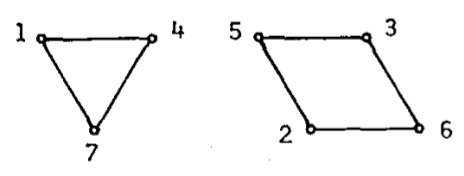
\includegraphics[width=0.3\textwidth]{images/1}& S_1:& \quad  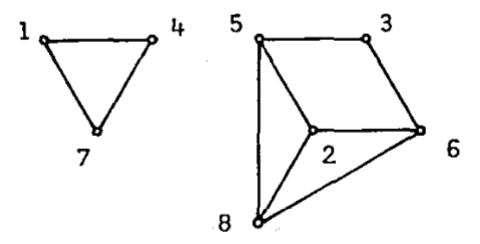
\includegraphics[width=0.3\textwidth]{images/2}\\
\end{align*}
\\ \\ \\
\begin{figure}[htb]
    \textbf{S:}
	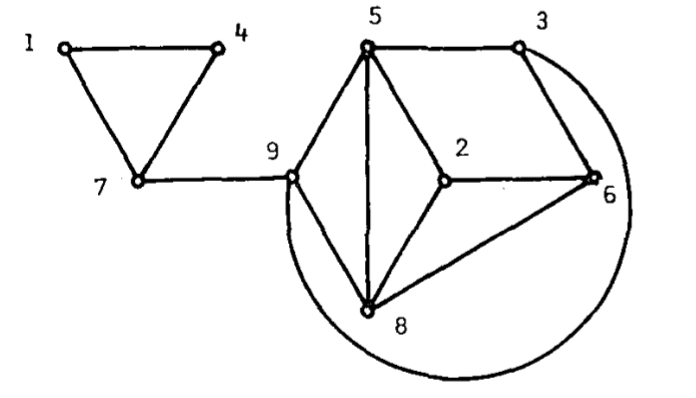
\includegraphics[width=0.65\textwidth]{images/3}
	\caption*{ Şekil 1.3.3 S tamsayılar dizisinin gerçekleştirimi }
	\label{fig:Bb}
\end{figure}\\ \\ \\
bu çizgeler arasında başka herhangi bir ilişki yoktur.
\end{document}